\documentclass[border=10pt]{standalone}
\usepackage{pgfplots}
\pgfplotsset{compat=1.18}
\begin{document}
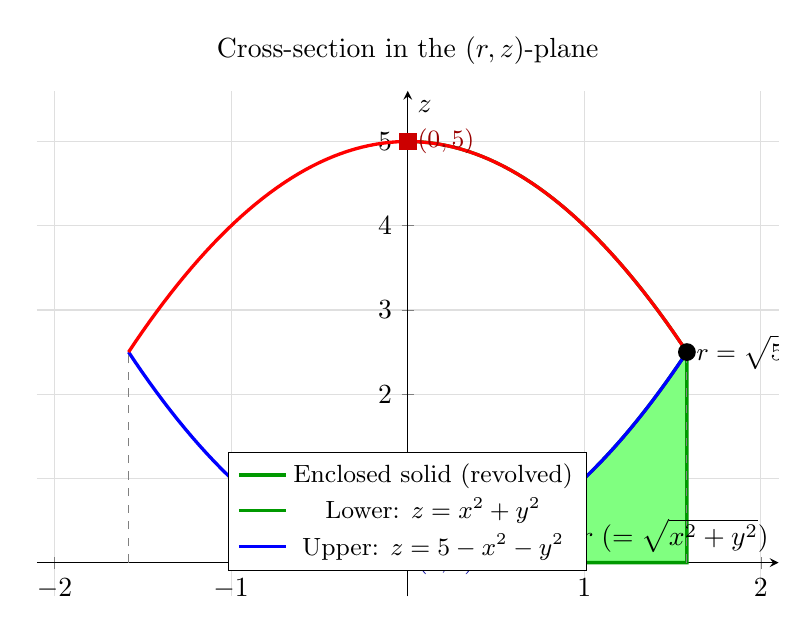
\begin{tikzpicture}
\begin{axis}[
    width=11cm, height=8cm,
    xlabel={$r \;(=\sqrt{x^2+y^2})$},
    ylabel={$z$},
    title={Cross-section in the $(r,z)$-plane},
    xmin=-2.1, xmax=2.1, ymin=-0.4, ymax=5.6,
    xtick={-2,-1,0,1,2}, ytick={0,1,2,3,4,5},
    grid=major, grid style={gray!25},
    legend style={at={(0.5,0.05)}, anchor=south, draw=black, font=\small},
    axis lines=middle,
]

% Fill the enclosed solid region (using parameterization)
\addplot[
    domain=0:1.5811388300841898,
    samples=80, fill=green!50, draw=green!60!black, very thick
] ({x}, {x^2}) \closedcycle;
% Add the upper edge of the enclosed region
\addplot[domain=0:1.5811388300841898, samples=80, draw=green!60!black, very thick] ({x}, {5-x^2});
\addlegendentry{Enclosed solid (revolved)}

% Lower paraboloid (full curve)
\addplot[domain=-1.5811:1.5811, samples=80, blue, very thick] {x^2};
\addlegendentry{Lower: $z = x^2+y^2$}

% Upper paraboloid (full curve)
\addplot[domain=-1.5811:1.5811, samples=80, red, very thick] {5-x^2};
\addlegendentry{Upper: $z = 5-x^2-y^2$}

% Intersection point
\addplot[only marks, mark=*, mark size=3pt, color=black] coordinates {(1.5811, 2.5)};
\node[anchor=west] at (axis cs:1.5811, 2.5)
    {\small $r=\sqrt{5/2},\; z=5/2$};

% Vertical dashed lines at intersection
\addplot[dashed, gray] coordinates {(1.5811, 0) (1.5811, 2.5)};
\addplot[dashed, gray] coordinates {(-1.5811, 0) (-1.5811, 2.5)};

% Apex of upper paraboloid
\addplot[only marks, mark=square*, mark size=3pt, color=red!80!black] coordinates {(0, 5)};
\node[anchor=west, red!60!black] at (axis cs:0, 5) {\small $(0,5)$};

% Apex of lower paraboloid
\addplot[only marks, mark=square*, mark size=3pt, color=blue!80!black] coordinates {(0, 0)};
\node[anchor=west, blue!60!black] at (axis cs:0, 0) {\small $(0,0)$};

\end{axis}
\end{tikzpicture}
\end{document}